\documentclass[12pt]{report}
\usepackage{styles/log-style}
\usepackage{setspace}  

\title{lab_report}
\author{Рамиль Титеев}
\date{September 2022}

\begin{document}
    \begin{titlepage}
        \begin{center}
            \large{Московский Aвиационный Институт}\\
            \large{(Национальный Исследовательский Университет)}\\
            \vspace{0.4in}
            \textbf{\LARGE{Факультет информационных технологий и прикладной математики}}\\
            \vspace{0.4in}
            \large{Кафедра вычислительной математики и программирования}\\
            \vspace{0.4in}
            \textbf{\LARGE{Лабораторная работa 1 по курсу ОOП:}}\\
            \textbf{\LARGE{основы программирования на языке С\#}}\\
        \end{center}
        \vspace{0.6in}
        \small{1.АГРЕГАЦИЯ ПО ССЫЛКЕ}\\
        \vfill
        \begin{flushleft}
                \large{ 
                    Работу выполнил:\\
                    М8О-205Б-21 \hspace{0.1in} 
                    Титеев Р.М. \hspace{0.3in}  
                    \tline{(\textit{подпись})}{\hspace{1in}} 
                    \hspace{0.3in} 
                    \tline{(\textit{вариант})}{\hspace{0.7in}}\\ 
                    Руководитель: \tline{(\textit{подпись})}{\hspace{1in}}/Кузнецова С.В. \\
                    Дата: \underline{\hspace{0.4in}} октября 2022\\
                }
        \end{flushleft}        
    \end{titlepage}

    \textbf{\large{Агрегация по ссылке}}\\
    \begin{center}
        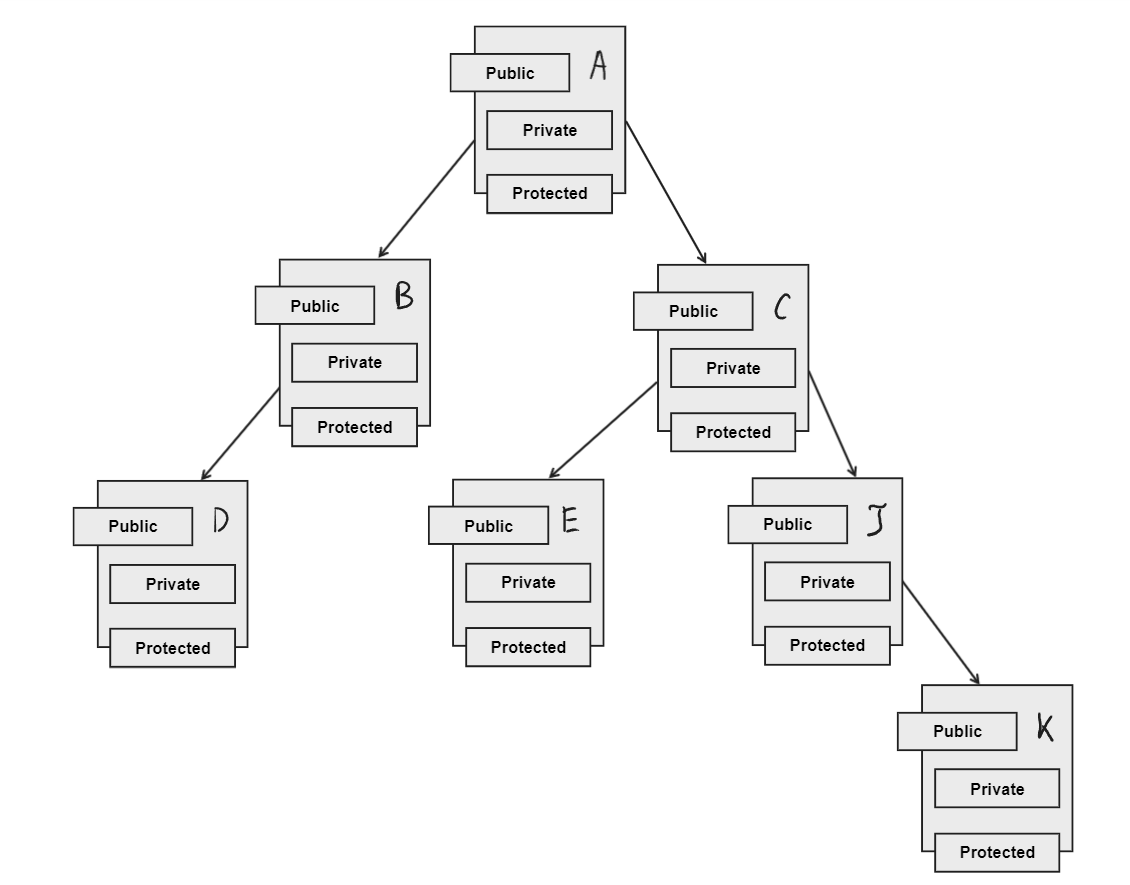
\includegraphics[scale=0.5]{formal/screen_2.png}\\
    \end{center}
    \textbf{Текст программы}\\
    \begin{lstlisting}[language={[Sharp]C}]
using System;
using System.Collections.Generic;
using System.Linq;
using System.Text;
using System.Threading.Tasks;

namespace lab_1
{
    class A
    {
        private B b = null;
        private C c = null;
        public A(B b, C c)
        {
            this.b = b;
            this.c = c;
        }
        public void mA()
        {
            Console.WriteLine("method of A");
        }
        public B bA
        {
            set { Console.WriteLine("set b"); b = value; }
            get { Console.Write("get b ->"); return b; }
        }
        public C cA
        {
            set { Console.WriteLine("set c"); c = value; }
            get { Console.Write("get c ->"); return c; }
        }
    }

    class B
    {
        private D d = null;
        public B(D d)
        {
            this.d = d;
        }
        public void mB()
        {
            Console.WriteLine(" method of B");
        }
        public D dA
        {
            set { Console.WriteLine("set d"); d = value; }
            get { Console.Write("get d ->"); return d; }
        }
    }

    class C
    {
        private J j = null;
        private E e = null;
        public C(J j, E e)
        {
            this.j = j;
            this.e = e;
            this.c_val = 10;
        }
        public void mC()
        {
            Console.WriteLine(" method of C");
        }
        public E eA
        {
            set { Console.WriteLine("set e"); e = value; }
            get { Console.Write("get e ->"); return e; }
        }
        public J jA
        {
            set { Console.WriteLine("set j"); j = value; }
            get { Console.Write("get j ->"); return j; }
        }
        public int c_val { set; get; }
    }

    class D
    {
        public D() { }
        public void mD()
        {
            Console.WriteLine(" method of D");
        }
    }

    class E
    {
        private D d = null;
        public E(D d)
        {
            this.d = d;
        }
        public void mE()
        {
            Console.WriteLine(" method of E");
        }

        public D dA
        {
            set { Console.WriteLine("set d"); d = value; }
            get { Console.Write("get d ->"); return d; }
        }
    }

    class J
    {
        private K k = null;
        public J(K k)
        {
            this.k = k;
        }
        public void mJ()
        {
            Console.WriteLine(" method of J");
        }

        public K kA
        {
            set { Console.WriteLine("set k"); k = value; }
            get { Console.Write("get k ->"); return k; }
        }
    }
    class K
    {
        public K() { }
        public void mK()
        {
            Console.WriteLine(" method of K");
        }
    }

    internal class Program
    {
        static void Main(string[] args)
        {
            K k = new K();
            D d = new D();
            E e = new E(d);
            J j = new J(k);

            B b = new B(d);
            C c = new C(j, e);

            A a = new A(b, c);

            Console.WriteLine($"Value in C before changes: {a.cA.c_val}");

            a.cA.c_val = 15;

            Console.WriteLine($"Value in C after changes: {a.cA.c_val}");

            Console.WriteLine();
            a.mA();
            a.bA.mB();
            a.cA.mC();

            a.bA.dA.mD();
            a.cA.eA.mE();
            a.cA.jA.mJ();

            a.cA.jA.kA.mK();
            Console.ReadKey();


        }
    }
}


\end{lstlisting}
    \vspace{0.4in}
    \textbf{Результат работы}\\
    \begin{center}
        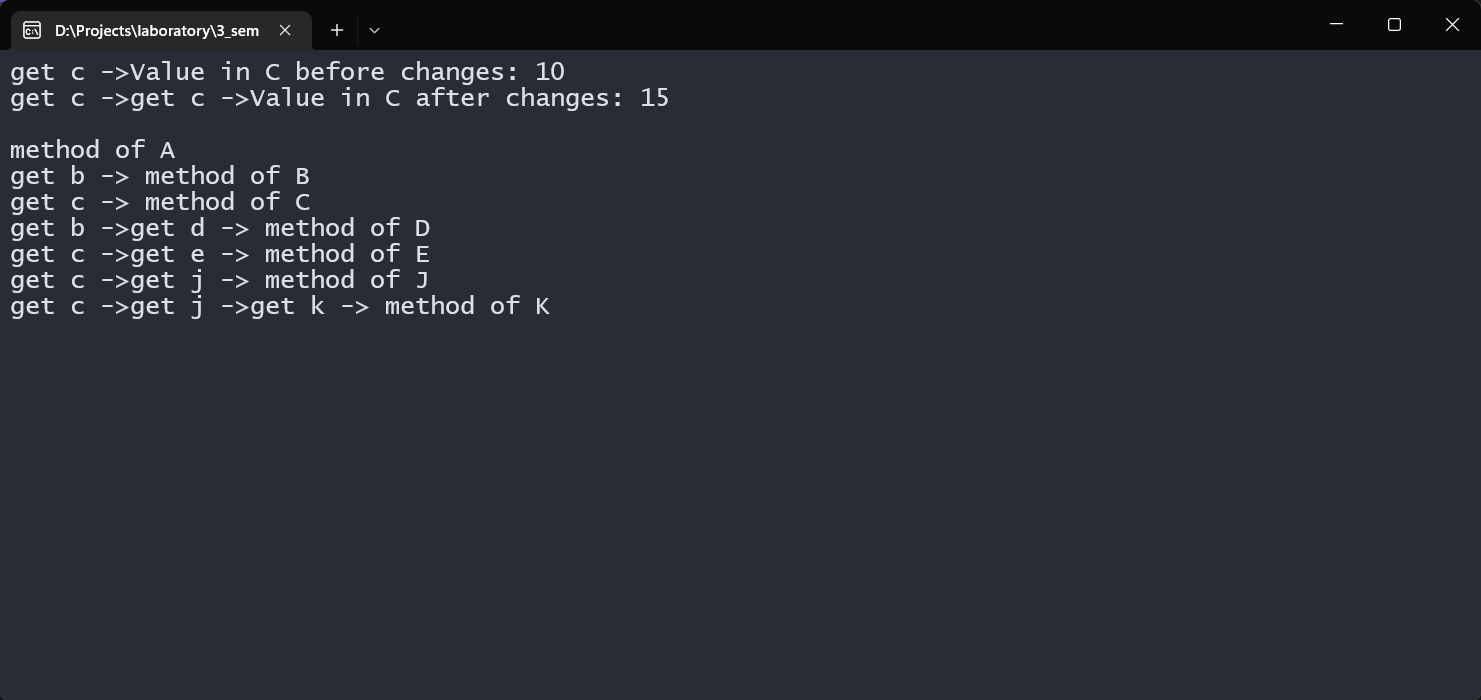
\includegraphics[scale=0.5]{formal/screen_1.png}\\
    \end{center}
    \textbf{Пример использования}\\
    Данный метод можно использовать в качестве описания структуры работников в какой-либо компании. 
    Так например есть главный класс и это будет главный человек в компании. Сначала мы инициализируем всех сотрудников 
    данной компании(при этом инициализация происходит по иерархии снизу вверх). Затем мы привязываем сотрудников к своим начальникам.
    Кроме этого, мы можем использовать уже проинициализированного работника в других целях, 
    и при этом его св-ва будут сохранятся в старой компании.
    \textbf{Вывод}\\
    Объекты классов A, B, C, D , E, J, K существуют независимо друг от друга. 
    При этом, например связывание объекта а с объектами b, c происходит с помощью конструктора; 
    b, c – параметры для конструктора A.
    Аналогичным образом происходит связывание $b$ c $d$, $c$ c $e$, $j$ и $j$  c $k$. 
    Но при этом объекты могут быть уничтожены по отдельности, что нарушает целостность структуры.

\end{document}
